
\documentclass[a4paper,14pt]{extarticle} 
\usepackage[T2A]{fontenc}
\usepackage[utf8]{inputenc} 
\usepackage{textcomp}
\usepackage[english,russian]{babel}
\usepackage{amssymb,amsfonts,amsmath,mathtext,enumerate} 
\usepackage{enumitem}
\usepackage{graphicx} 
\usepackage{cmap}
\usepackage{array}
\usepackage[usenames]{color}
\usepackage{multirow,makecell,array}

\newcommand*\rot{\rotatebox{90}}
\newcommand*\OK{\ding{51}}
\newcommand{\tabitem}{~~\llap{\textbullet}~~}

\renewcommand{\baselinestretch}{1.5} 
\usepackage{indentfirst}
\sloppy					
\clubpenalty=10000		
\widowpenalty=10000

\newcommand*{\hm}[1]{#1\nobreak\discretionary{}% Перенос знаков в формулах
	{\hbox{$\mathsurround=0pt #1$}}{}}


 \usepackage[unicode]{hyperref} % Гиперссялки
 \hypersetup{
 	colorlinks = true,
 	linkcolor = [rgb]{0, 0.2, 0.9},
 	urlcolor = [rgb]{0,0,1},
 	citecolor = red
 }

\DeclareGraphicsExtensions{.pdf,.png,.jpg}
\usepackage{setspace}

\usepackage{tikz}
\usetikzlibrary{arrows.meta}
\usetikzlibrary{positioning}

\DeclareMathOperator*{\tg1}{tg}

\usepackage{geometry} 
\geometry{left=3cm}
\geometry{right=1.5cm}
\geometry{top=2cm}
\geometry{bottom=2cm}


\usepackage{fancyhdr}


\usepackage[backend=biber,bibencoding=utf8,sorting=none,maxcitenames=3,style=gost-numeric]{biblatex}


\usepackage{stringenc}
\usepackage{pdfescape}

\makeatletter
\renewcommand*{\UTFviii@defined}[1]{%
  \ifx#1\relax
    \begingroup
      % Remove prefix "\u8:"
      \def\x##1:{}%
      % Extract Unicode char from command name
      % (utf8.def does not support surrogates)
      \edef\x{\expandafter\x\string#1}%
      \StringEncodingConvert\x\x{utf8}{utf16be}% convert to UTF-16BE
      % Hexadecimal representation
      \EdefEscapeHex\x\x
      % Enhanced error message
      \PackageError{inputenc}{Unicode\space char\space \string#1\space
                              (U+\x)\MessageBreak
                              not\space set\space up\space
                              for\space use\space with\space LaTeX}\@eha
    \endgroup
  \else\expandafter
    #1%
  \fi
}
\makeatother

\DeclareUnicodeCharacter{0306}{}
\DeclareUnicodeCharacter{FFFC}{}

\makeatletter
\patchcmd{\l@section}{\hfil}{%
  \leaders\hbox{$\m@th
    \mkern \@dotsep mu\hbox{.}\mkern \@dotsep
  mu$}\hfill}{}{}
\makeatother

\begin{document}

\begin{titlepage}
\begin{center}
{\normalsize АВТОНОМНАЯ НЕКОММЕРЧЕСКАЯ ОРГАНИЗАЦИЯ} \\ 
{\normalsize <<РЕГИОНАЛЬНАЯ АНАЛИТИКА>>} \\
\vspace{\baselineskip}
\vspace{\baselineskip}
\vspace{\baselineskip}
\vspace{\baselineskip}
\vspace{\baselineskip}
\vspace{\baselineskip}
\vspace{\baselineskip}
\vspace{\baselineskip}
\vspace{\baselineskip}
{\LARGE АНАЛИТИЧЕСКИЙ ОТЧЕТ} \\
\vspace{10mm}
{\huge \textbf{ Интернет-портрет региона \\ {{content}} } } \\
\vspace{\baselineskip}
\vspace{80mm}
\today \\
{Москва} 
\end{center}
\end{titlepage}
\newpage
\tableofcontents 
\newpage
\section{Введение}
\subsection{Необходимость анализа СМИ}
При формировании бренда территории необходимо учитывать множество факторов, которые могут повлиять на развитие территории. Одним из ключевых факторов при этом является создаваемый в средствах массовой информации образ региона. 

Важность данного фактора связана с тем, что сегодня все экономические агенты имеют равный доступ к информационным ресурсам, а СМИ являются основным каналом трансляции информации. Основываясь на данных, полученных из различных источников, формируется общественное мнение о регионе. Тем самым создание и поддержание позитивного образа территории в СМИ позволяет, прежде всего, привлекать инвестиции, расширять рынки сбыта продукции национальных производителей, привлекать трудовые ресурсы и развивать туризм – то есть поддерживать развитие столь важных в регионе отраслей.

Роль СМИ значительно увеличивается при необходимости построения или коррекции имиджа территории. Стоит отметить, что искусственно созданный имидж территории может не отражать, например, основополагающих социальных и экономических характеристик, противоречий территории, реальных принципов и методов ведения национального/регионального бизнеса, особенностей жизни населения, влияния экономики территории на окружающую среду и т.д., тем самым отвлекать внимание общественности от проблем территории.

Однако чаще всего регионы сталкиваются с проблемой формирования у общественности стереотипного мнения о характеристиках объекта на основе одной существующей (или существовавшей ранее) особенности региона. Таким образом, администрация региона сталкивается с тем, что формируемый имидж территории в СМИ извне часто отличается от того, что  стремятся сформировать внутри региона. В связи с этим возникает необходимость оценки реального образа региона в СМИ извне. 

\newpage
\section{Анализ информационного пространства}

\subsection{Основные параметры отчета}
Проведен анализ новостей по следующей конфигурации:

\begin{itemize} 
  \item Начальная дата: \textbf{ {{period_from}} }
  \item Конечная дата: \textbf{ {{period_to}} }
  \item Регион: \textbf{ {{content}} }
  \item Количество источников: \textbf{ {{number_of_sources}} }
	\item Количество новостей: \textbf{ {{number_of_news}} }
\end{itemize}
\includegraphics[width=\textwidth]{{ '{' }}{{ map_path }}{{ '}' }}


\newpage
\subsection{Ключевые события}
Наиболее важные события за данный период:
  \begin{itemize}
    
      \item \textbf{ {{ title }} } -- {{ num_sources }} источников. \\
      \includegraphics[width=0.72\textwidth]{{ '{' }}{{ img_path }}{{ '}' }}
    
  \end{itemize}
 

\newpage

Общий график частот встречаемости топ-10 новостей с наибольшим количеством источников:
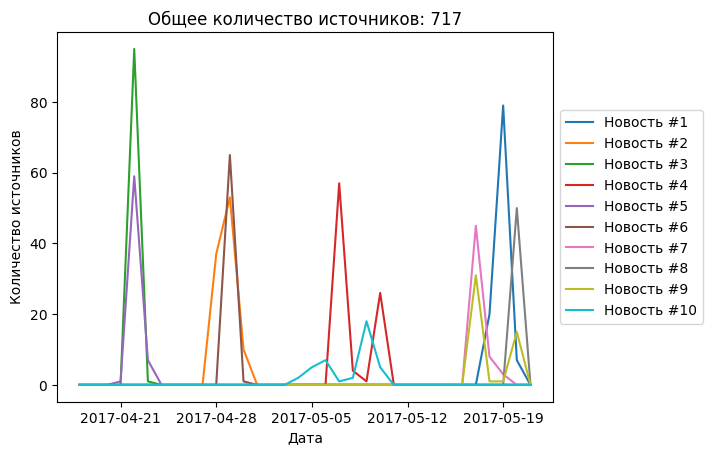
\includegraphics[width=\textwidth]{all_news.png}

\newpage
\subsection{Ключевые слова}
Для выделения основных слов и понятий используется технология построения облака тэгов. Для региона {{ content }} облако тэгов, построенное по заголовком новостных событий выглядит следующим образом:

\begin{figure}[h!]
\centering
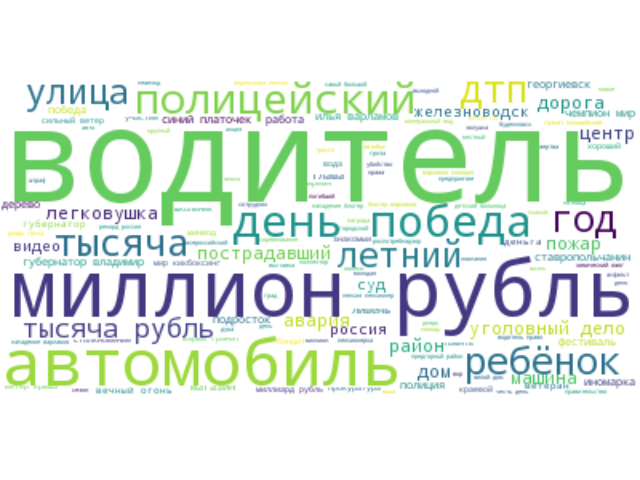
\includegraphics[width=\textwidth]{wordcloud.png}
\end{figure}

\newpage
Ниже приведена таблица, состоящая из 10 слов с наибольшей частотой встречаемости в заголовках:

\begin{center}
\begin{tabular}{ |c|c|c| } 
 \hline
\textbf{Слово} & \textbf{Частота вхождения в заголовки} \\ 

    \hline
    {{ word }} & {{ frequency }} \\

 \hline
\end{tabular}
\end{center}

\newpage
\subsection{Граф связей слов}

Построим общую схему новостного пространства региона {{ content }} для топ 5\% словосочетаний по встречаемости:

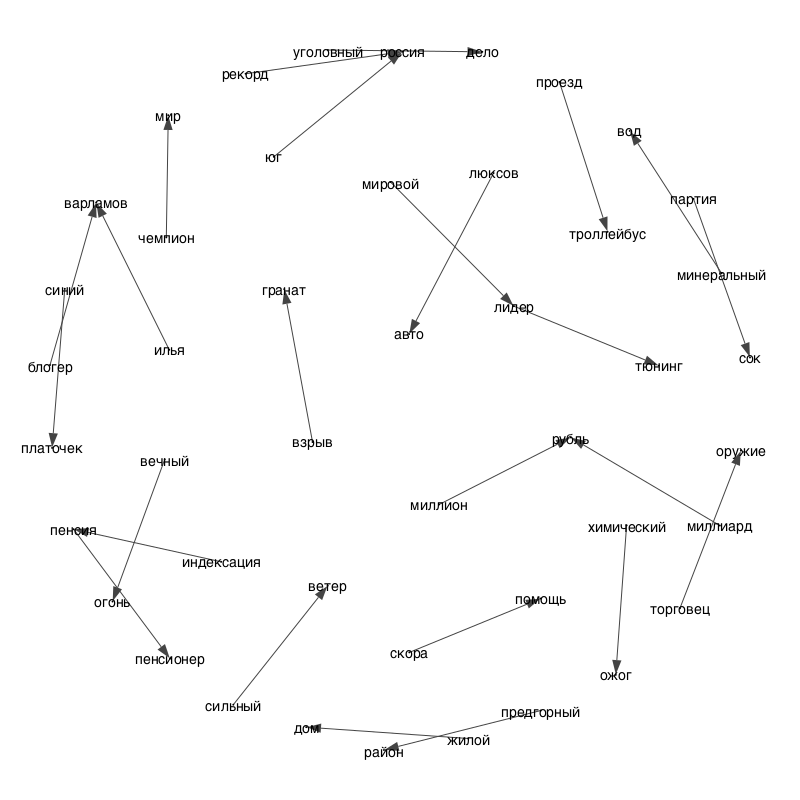
\includegraphics[width=\textwidth]{graph1.png}

\newpage

\section{Обработка данных Авито}

\subsection{Необходимость анализа рынка услуг}

В данной главе проведен анализ рынка услуг по объявлениям с сайта <<Авито>> в категории \textbf{<<Услуги>>}.

В качестве основных методов для исследования были выбраны:
\begin{itemize}
\item автоматическое разбиение объявлений по категориям
\item анализ и представление основных понятий и терминов в виде облака тэгов. 
\end{itemize}

\subsection{Анализ объявлений}
Проведя анализ  {{ avito_total }} топиков avito за заданный период мы можем получить следующую статистику:

\begin{enumerate}
  
    \item Найдено {{ frequency }} услуг в категории \textbf{ {{ topic }} } \\
    \includegraphics[width=0.9\textwidth]{{ '{' }}{{ img_path }}{{ '}' }}
  
  
\end{enumerate}

\newpage

\section{Заключение}
В данном отчете был проведен анализ событийного фона региона {{ content }} с точки зрения внешнего наблюдателя. Также, был проведен анализ рынка услуг в регионе по данным сайта <<Авито>>. 
\newpage

\begin{thebibliography}{9}
\bibitem{yandex} 
<<Яндекс-новости>>. 
\textit{https://news.yandex.ru/}, 21.05.2017.
\bibitem{avito} 
<<Авито>>. 
\textit{https://avito.ru/}, 21.05.2017.
\end{thebibliography}

\end{document}

